\chapter{Probability Model}\label{S:ProbModel}

\section{Experiments}\label{S:Experiments}

Ideas about chance events and random behaviour arose out of thousands of
years of game playing, long before any attempt was made to use
mathematical reasoning about them. Board and dice games were well known
in Egyptian times, and Augustus Caesar gambled with dice. Calculations
of odds for gamblers were put on a proper theoretical basis by Fermat
and Pascal in the early 17th century.

\begin{definition}
An {\bf experiment} is an activity or procedure that produces distinct, well-defined possibilities called {\bf outcomes}.  
The set  of all outcomes   is called the {\bf sample space}, and is denoted by $\Omega$.

The subsets of $\Omega$ are called {\bf events}.  
A single outcome, $\omega$, when seen as a subset of $\Omega$, as in
$\{\omega\}$, is called a  {\bf simple event}.

Events, $E_1,\, E_2\, \dots \, E_n$,  that cannot occur at the same time are called {\bf mutually exclusive} events, or {\bf pair-wise disjoint} events.  This means that $E_i
\cap E_j = \emptyset $ where $i\not=j$.
\end{definition}



\begin{example}
Some standard examples of experiments are the following:

\bit

\item $\Omega=\{ {\textsf{Defective, Non-defective}} \}$ if our
  experiment is to inspect a light bulb.

There are only two outcomes here, so   $\Omega = \{ \omega_1, \omega_2\}$
where $\omega_1= {\textsf{Defective}}$ and  $\omega_2 =
{\textsf{Non-defective}}$.


\item $\Omega=\{ {\textsf{Heads, Tails}} \}$ if our experiment is to
  note the outcome of a coin toss.


This time, $\Omega=\{ \omega_1, \omega_2\}$ where $\omega_1= {\textsf{Heads}}$ and  $\omega_2 = {\textsf{Tails}}$.


\item If our experiment is to roll a die  then there are six outcomes corresponding to
  the number that shows on the top. For this experiment,
  $\Omega = \{\mathsf{1,2,3,4,5,6}\}$.


Some examples of events are the set of odd numbered outcomes
$A=\{\mathsf{1,3,5}\}$, and  the set of
even numbered outcomes $B=\{\mathsf{2,4,6}\}$.


The simple events  of $\Omega$ are $\{\sf{1}\}, \{\sf{2}\}, \{\sf{3}\}, \{\sf{4}\}, \{\sf{5}\}$, and $\{\sf{6}\}$.

\eit
\end{example}


The outcome of a random experiment is uncertain until it is performed and observed.  
Note that sample spaces need to reflect the problem in hand.  
The example below is to convince you that an experiment's sample space is merely a collection of distinct elements called outcomes and these outcomes have to be {\em discernible in some well-specified sense} to the experimenter!


\begin{example}
\label{Eg:SensoryDiscerningExperiments} 
Consider a generic
  die-tossing experiment by a human experimenter. Here \newline $\Omega=
  \{\omega_1,\omega_2,\omega_3,\ldots,\omega_6\}$, but the
  experiment might correspond to rolling a die whose faces are:
\begin{enumerate}
\item sprayed with six different scents (nose!), or
\item studded with six distinctly flavoured candies (tongue!), or
\item contoured with six distinct bumps and pits (touch!), or
\item acoustically discernible at six different frequencies (ears!), or
\item painted with six different colours (eyes!), or
\item marked with six different numbers $\mathsf{1,2,3,4,5,6}$ (eyes!), or , \ldots
\end{enumerate}
These six experiments are  equivalent as far as probability goes.
\end{example}


\begin{definition}
{A {\bf trial} is a single performance of an experiment and it
  results in an outcome.}
\end{definition}



\begin{example}
Some standard examples of a trial are:

\bit

\item A roll of a die.

\item A toss of a coin.

\item A release of a chaotic double pendulum.

\eit
\end{example}

An experimenter often performs more than one trial.  Repeated trials of an experiment forms the basis of science and engineering as the experimenter learns about the phenomenon by repeatedly performing the same mother experiment with possibly different outcomes.  This repetition of trials in fact provides the very motivation for the definition of probability.

\begin{definition}{An {\bf ${\mathbf n}$-product experiment} is obtained by
    repeatedly performing $n$ trials of some experiment. 
    %This experiment is often called the mother experiment.% Raaz substituted to avoid the ambiguous reference to 'This'
    The experiment that is repeated is called the ``mother'' experiment.}
\end{definition}



\begin{example}[Toss a coin $n$ times]\label{EX:T3X}
Suppose our experiment entails tossing a coin $n$ times and recording ${\tt H}$ for Heads and ${\tt T}$ for Tails.  When $n=3$, one possible outcome of this experiment is ${\tt HHT}$, ie.~a Head followed by another Head and then a Tail.  Seven other outcomes are possible.  
%Below, we refer to this experiment by the symbol $\E{E}_{\theta}^{3}$.  More generally, we refer to the experiment of tossing a coin $n$ times as $\E{E}_{\theta}^{n}$ and sometimes refer to $\E{E}_{\theta}^{1}$ by $\E{E}_{\theta}$ for simplicity.  The reason for the $\theta$ subscrip will become apparent as we develop the theory.
\end{example}


The sample space for ``toss a coin three times" experiment %$\E{E}_{\theta}^{3}$ %\hyperref[EX:T3X]{Experiment \ref*{EX:T3X}} of tossing a coin 3 times 
is:
\[
\Omega = \{ {\tt H}, {\tt T} \}^3 =  \{ {\tt HHH}, {\tt HHT}, {\tt HTH}, {\tt HTT}, {\tt THH}, {\tt THT}, {\tt TTH}, {\tt TTT}  \} \ ,
\]
with a particular sample point or outcome $\omega = {\tt HTH}$, and another distinct outcome $\omega' = {\tt HHH}$.  An event, say $A$, that `at least two Heads occur' is the following subset of $\Omega$:
\[
A = \{ {\tt HHH}, {\tt HHT}, {\tt HTH}, {\tt THH} \} \ .
\]
Another event, say $B$, that `no Heads occur' is:
\[
B = \{{\tt TTT}\}
\]
Note that the event $B$ is also an outcome or sample point.  Another interesting event is the empty set $\emptyset  \subset \Omega$.  The event that `nothing in the sample space occurs' is $\emptyset$.

\begin{classwork}[A thrice-bifurcating tree of outcomes]
Can you think of a graphical way to enumerate the outcomes of the Experiment~\ref{EX:T3X}%$\E{E}_{\theta}^{3}$
?  Draw a diagram of this under the caption of \hyperref[F:T3X]{Figure~\ref*{F:T3X}}, using the caption as a hint (in other words, draw your own \hyperref[F:T3X]{Figure~\ref*{F:T3X}}).
\begin{figure}[htpb]
\caption{A binary tree whose leaves are all possible outcomes.\label{F:T3X}}
\vspace{4cm}
\end{figure}
\end{classwork}

\remove{
In \hyperref[LW:T3X]{Labwork~\ref*{LW:T3X}} we implement \hyperref[AL:T3X]{Algorithm~\ref*{AL:T3X}} to  print all the outcomes.  The algorithm uses {\bf for loops} to reach the leaves (outcomes of $\E{E}_{\theta}^{3}$) of the binary tree.
\begin{algorithm}[htpb]
\caption{List $\Omega$ for ``Toss a Coin Three Times" experiment $\E{E}_{\theta}^{3}$}
\label{AL:T3X}
\begin{algorithmic}[1]
\STATE {\it input:} nothing

\STATE {\it output:} print/list all outcomes of $\E{E}_{\theta}^{3}$ 

\STATE {\it initialize:} ${\bf SampleSpace1Toss} = \{ {\tt H}, {\tt T} \}$  \COMMENT{{\tiny ${\bf SampleSpace1Toss}[1]={\tt H}$ and ${\bf SampleSpace1Toss}[2]={\tt T}$}}
\FOR{$i=1$ to $2$} 
\FOR{$j=1$ to $2$}
\FOR{$k=1$ to $2$}
\STATE {
 Print ${\bf SampleSpace1Toss}[i]$ ${\bf SampleSpace1Toss}[j]$ ${\bf SampleSpace1Toss}[k]$ \\
Print `` , "  \COMMENT{{\tiny print a comma character to delimit outcomes}}
}
\ENDFOR
\ENDFOR
\ENDFOR
\end{algorithmic}
\end{algorithm}

\begin{labwork}[Three for loops for the thrice-bifurcating tree]\label{LW:T3X}
Let's write a {\sc Matlab} code in a script file named {\tt OutcomesOf3Tosses.m} that implements \hyperref[AL:T3X]{Algorithm~\ref*{AL:T3X}} to print all the outcomes of $\E{E}_{\theta}^{3}$.  You need to go to the File menu and create a new file named {\tt OutcomesOf3Tosses.m} Run it in the command window.
\begin{VrbM}
>> type OutcomesOf3Tosses.m

SampleSpace1Toss='HT';	% declare a string vector or character array
% SampleSpace1Toss is the name of the char array
SampleSpace1Toss(1);		% access the first element 'H' this way
SampleSpace1Toss(2);		% access the second element 'T' this way
% Now let's write the routine for listing the sample space of 'toss 3 times'
w=' ';		% declare w to be the character ' '
for i = 1:1:2		% for loop for variable i = start:increment:end
  for j = 1:1:2		% for loop for variable j
    for k = 1:1:2	% for loop for variable j
     % next we concatenate using strcat -- strcat('A','B','C','D') concatenates the 4 char arrays
     x = strcat(SampleSpace1Toss(i),SampleSpace1Toss(j),SampleSpace1Toss(k),' , '); % ' ,' delimited outcome
     w = strcat(w,x); % recursively store the outcomes in a new array w
    end
  end
end
w		% print w at the end of the three for loops
>> lab1work4
>> SampleSpace1Toss(1)
ans = H
>> SampleSpace1Toss(2)
ans = T
>> w
w = HHH ,HHT ,HTH ,HTT ,THH ,THT ,TTH ,TTT ,
\end{VrbM}
\end{labwork}
}


\begin{framed}
EXPERIMENT SUMMARY\\

\begin{tabular}{rcl}
Experiment &$-$& an activity producing distinct outcomes.\\
$\Omega$ &$-$& set of all outcomes of the experiment.\\
$\omega$ &$-$& an individual outcome in $\Omega$, called a simple event.\\
$A\subseteq \Omega$ &$-$& a subset $A$ of $\Omega$ is an event.\\
Trial &$-$& one performance of an experiment resulting in 1 outcome.\\
\end{tabular}
\end{framed}


\section{Probability}\label{S:Probability}
The  mathematical model for probability or the probability model is an axiomatic system that may be motivated by the intuitive idea of `long-term relative frequency'.  If the axioms and definitions are intuitively motivated, the probability model simply follows from the application of logic to these axioms and definitions.  No attempt to define probability in the real world is made. However, the application of probability models to real-world problems through statistical experiments has a fruitful track record.  In fact, you are here for exactly this reason.

\begin{idea}[The long-term relative frequency (LTRF) idea]
Suppose we are interested in the fairness of a coin, i.e.~if landing Heads has the same ``probability" as landing Tails.  We can toss it $n$ times and call 
$N({\tt H},n)$ the fraction of times we observed Heads out of $n$ tosses.
Suppose that after conducting the tossing experiment $1000$ times, we rarely observed Heads, e.g.~$9$ out of the $1000$ tosses, then $N({\tt H},1000)=9/1000=0.009$.  Suppose we continued the number of tosses to a million and found that this number approached closer to $0.1$, or, more generally, $N({\tt H},n) \to 0.1$ as $n \to \infty$.  We might, at least intuitively, think that the coin is unfair and has a lower ``probability'' of $0.1$ of landing Heads.  We might think that it is fair had we observed $N({\tt H},n) \to 0.5$ as $n \to \infty$.  Other crucial assumptions that we have made here are:
\begin{enumerate}
\item {\bf Something Happens}: Each time we toss a coin, we are certain to observe Heads {\bf or} Tails, denoted by ${\tt H} \cup {\tt T}$.  The probability that ``something happens'' is $1$.  More formally:
\[
N({\tt H} \cup {\tt T},n)= \frac{n}{n} = 1.
\]
This is an intuitively reasonable assumption that simply says that one of the possible outcomes is certain to occur, provided the coin is not so thick that it can land on or even roll along its circumference.

\item {\bf Addition Rule}: Heads and Tails are mutually exclusive events in any given toss of a coin, i.e.~they cannot occur simultaneously.  The intersection of mutually exclusive events is the empty set and is denoted by ${\tt H} \cap {\tt T} = \emptyset$. The event ${\tt H} \cup {\tt T}$, namely that the event that ``coin lands Heads {\bf or} coin lands Tails" satisfies:
\[
N({\tt H} \cup {\tt T},n)= N({\tt H},n) + N({\tt T},n) .
\]
\item The coin-tossing experiment is repeatedly performed in an {\bf independent} manner, i.e.~the outcome of any individual coin-toss does not affect that of another.  This is an intuitively reasonable assumption since the coin has no memory and the coin is tossed identically each time.
\end{enumerate}
\end{idea}

We will use the LTRF idea more generally to motivate a mathematical model of probability called probability model.  Suppose $A$ is an event associated with some experiment $\E{E}$, so that $A$ either does or does not occur when the experiment is performed.  We want the probability that event $A$ occurs in a specific performance of $\E{E}$, denoted by $\p(A)$, to intuitively mean the following:  if one were to perform a super-experiment $\E{E}^{\infty}$ by independently repeating the experiment $\E{E}$ and recording $N(A,n)$, the fraction of times $A$ occurs in the first $n$ performances of $\E{E}$ within the super-experiment $\E{E}^{\infty}$. Then the LTRF idea suggests:
\begin{equation}\label{E:NofAn}
N(A,n) :=  \frac{\text{Number of times $A$ occurs}}{n=\text{Number of performances of $\E{E}$}} \to \p(A), \ as \quad  n \to \infty
\end{equation}

Now, we are finally ready to define probability.
\begin{definition}[Probability]\label{D:Prob}
Let $\E{E}$ be an experiment with sample space $\Omega$.  Let $\C{F}$ denote a suitable collection of events in $\Omega$ that satisfy the following conditions:
\begin{enumerate}
\item It (the collection) contains the sample space:
$\boxed{
\Omega \in \C{F} }$.
\item It is closed under complementation:
$\boxed{
A \in \C{F} \quad \implies \quad A^c \in \C{F} }$.
\item It is closed under countable unions:
$\boxed{
A_1, A_2, \ldots \in \C{F} \quad \implies \quad \bigcup_{i} {A_i} := A_1 \cup A_2 \cup \cdots \in \C{F} }$.
\end{enumerate}
Formally, this collection of events is called a {\bf sigma field} or a {\bf sigma algebra}.  Our experiment $\E{E}$ has a sample space $\Omega$ and a collection of events $\C{F}$ that satisfy the three condition. 

Given a double, e.g. $(\Omega, \C{F})$, {\bf probability} is just a function $\p$ which assigns each event $A \in \C{F}$ a number $\p(A)$ in the real interval $[0,1]$, i.e.~$\boxed{\p : \C{F} \to [0,1] }$, such that:
\begin{enumerate}
\item The `Something Happens' axiom holds, i.e.~$\boxed{\p(\Omega) = 1}$. 
\item The `Addition Rule' axiom holds, i.e.~for events $A$ and $B$:
$$
\boxed{
A \cap B = \emptyset \quad \implies \quad \p(A \cup B) = \p(A) + \p(B)
} \ .
$$
\end{enumerate}
\end{definition}
\subsection{Consequences of our Definition of Probability}\label{S:ConseqDefProb}
It is important to realize that we accept the `addition rule' as an axiom in our mathematical definition of probability (or our probability model) and we do {\bf not} prove this rule.  However, the facts which are stated ({\scriptsize with proofs}) below, are logical consequences of our definition of probability:
\begin{enumerate}
\item For any event $A$, $\boxed{\p(A^c) = 1 - \p(A)}$.
{\scriptsize
\begin{proof}
One line proof.
\[
\overbrace{\p(A) + \p(A^c)}^{LHS} \underbrace{=}_{+~\text{rule}~\because A \cap A^c = \emptyset} \p(A \cup A^c) \underbrace{=}_{A \cup A^c = \Omega} \p(\Omega) \underbrace{=}_{\because~\p(\Omega) = 1} \overbrace{1}^{RHS} \quad \underbrace{\Longrightarrow}_{LHS-\p(A)~\&~RHS-\p(A)} \quad \p(A^c) = 1-\p(A)
\]
\end{proof}
}
\begin{itemize}
\item If $A = \Omega$ then $A^c = \Omega^c = \emptyset$ and 
$\boxed{\p(\emptyset) = 1-\p(\Omega) = 1-1 = 0}$.
\end{itemize}

\item For any two events $A$ and $B$, we have the {\bf inclusion-exclusion principle}:
\[
\boxed{
\p(A \cup B) = \p(A) + \p(B) - \p(A \cap B)
}.
\]
{\scriptsize
\begin{proof}
Since: 
\begin{eqnarray}
\quad A = (A \setminus B) \cup (A \cap B) & \quad \text{and} \quad & (A \setminus B) \cap (A \cap B) = \emptyset, \notag \\
\quad A \cup B = (A \setminus B) \cup B & \quad \text{and} \quad & (A \setminus B) \cap B = \emptyset \notag
\end{eqnarray}
the addition rule implies that:
\begin{eqnarray}
\p(A) &=& \p(A \setminus B) + \p(A \cap B) \notag \\
\p(A \cup B) &=& \p(A \setminus B) + \p(B) \notag
\end{eqnarray}
Substituting the first equality above into the second, we get:
\[
\p(A \cup B) = \p(A \setminus B) + \p(B) = \p(A) - \p(A \cap B) + \p(B)
\]
\end{proof}
}
\item From inclusion-exclusion principle we get {\bf Boole's inequality}: for any two events $A, B$
\[
\p(A \cup B) \leq \p(A) + \p(B)
\]
\item The inclusion-exclusion principle extends similarly to any three events $A_1,A_2,A_3$ as follows:
\[
\p(A_1 \cup A_2 \cup A_3) = \p(A_1) + \p(A_2) + \p(A_3) - \p(A_1 \cap A_2) - \p(A_1 \cap A_3) - \p(A_2 \cap A_3) + \p(A_1 \cap A_2 \cap A_3)
\]
and generalises to any $n$ events $A_1,A_2,\ldots,A_n$ as folows:
\[
\p \left( \bigcup_{i=1}^n A_i \right) = \sum_{i=1}^n \p(A_i) - \sum_{i<j} \p(A_i \cap A_j) + \sum_{i<j<k} \p(A_i \cap A_j \cap A_k) + \cdots + (-1)^{n-1} \sum_{i< \cdots <n} \p \left( \bigcap_{i=1}^n A_i \right)
\]

{\scriptsize
\begin{proof} See the counting argument in \url{https://en.wikipedia.org/wiki/Inclusion\%E2\%80\%93exclusion_principle} if you are curious.
\end{proof}
}  
\item Once again by the inclusion-exclusion principle, the Boole's inequality generalises to any $n$ events $A_1,A_2,\ldots,A_n$ as folows:
\[
\p \left( \bigcup_{i=1}^n A_i \right) \leq \sum_{i=1}^n \p(A_i)
\]
\item For a sequence of mutually disjoint events $A_1, A_2, A_3, \ldots, A_n$: 
\[
\boxed{
A_i \cap A_j = \emptyset \quad \text{for any $i \neq j$} \quad \implies \quad \p(A_1 \cup A_2 \cup \cdots \cup A_n) = \p(A_1)+\p(A_2)+ \cdots + \p(A_n)} .
\]
{\scriptsize
\begin{proof}
If $A_1, A_2, A_3$ are mutually disjoint events, then $A_1 \cup A_2$ is disjoint from $A_3$.  Thus, two applications of the addition rule for disjoint events yields:
\[
\p(A_1 \cup A_2 \cup A_3) = \p((A_1 \cup A_2) \cup A_3) \underbrace{=}_{+~\text{rule}} \p(A_1 \cup A_2) + \p(A_3) \underbrace{=}_{+~\text{rule}}  \p(A_1) + \p(A_2) + \p(A_3)
\]
The $n$-event case follows by mathematical induction.
\end{proof}
}
\end{enumerate}

We have formally defined the {\bf probability model} specified by the {\bf probability triple} $(\Omega, \C{F},\p)$ that can be used to model an {\bf experiment} $\E{E}$.

\begin{example}[First Ball out of NZ Lotto]\label{Eg:NZLottoModel}
Let us observe the number on {\em the first ball that pops out in a New Zealand Lotto trial}.  
There are forty balls labelled $1$ through $40$ for this experiment and so the sample space is \[\Omega\;=\;\{\mathsf{1,2,3,\dots,39,40}\}\,.\]  
Because the balls are vigorously whirled around inside the Lotto machine, modelled as a well-stirrred urn, before the first one pops out, 
we can model each ball to pop out first with the same probability. 
So, we assign each outcome $\omega \in \Omega$ the same probability of $\frac{1}{40}$, i.e., our probability model for this experiment is:
\[
\p(\omega) = \frac{1}{40}, \ \text{for each \ } \omega \in \Omega = \{\mathsf{1,2,3,\ldots,39,40}\} \enspace .
\]
Note: We sometimes abuse notation and write $\p(\omega)$ instead of the
more accurate but cumbersome $\p(\{\omega\})$ when writing down
probabilities of simple events. 

Crucially, by $\omega=\mathsf{17}$ for example, we mean all the detailed dynamics inside the Lotto machine that lead to the event that the ball labelled by the number $\mathsf{17}$ ends up popping out. 
So, $\Omega$ here is indeed a more complicated set although it only leads to $40$ possible outcomes.

Figure~\ref{F:LottoDraws}~(a) shows the frequency of the first ball number in 1114 NZ Lotto draws.  
Figure~\ref{F:LottoDraws}~(b) shows the relative frequency, i.e., the frequency divided by $1114$, the number of draws.  
Figure~\ref{F:LottoDraws}~(b) also shows the equal probabilities under our model.

\begin{figure}[htbp]
\centering
\subfigure[{\scriptsize Frequency of first ball.}]{
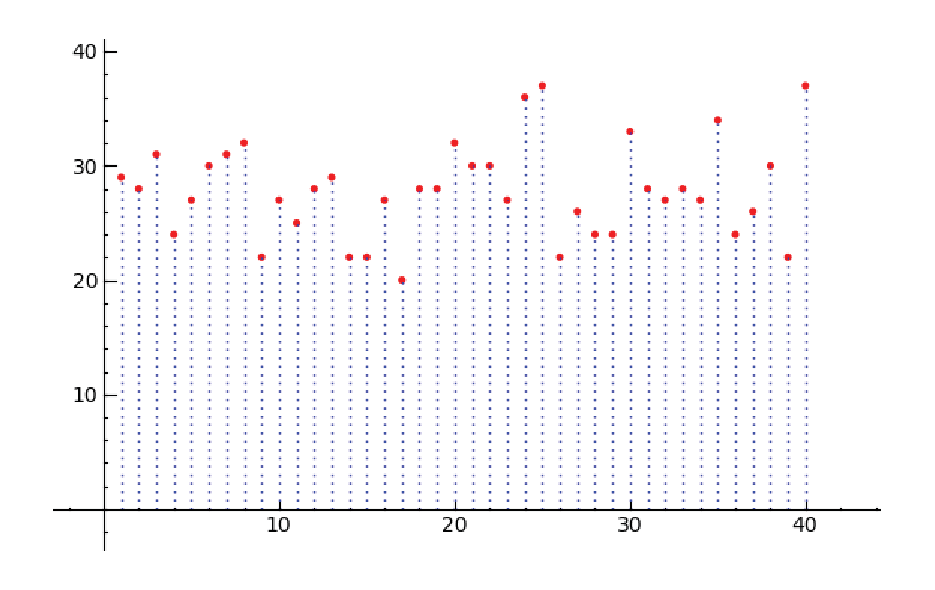
\includegraphics[width=7.5cm,height=4cm]{figures/mylotto_freq}}
\quad
\subfigure[{\scriptsize Relative frequency and probability of first ball.}]{
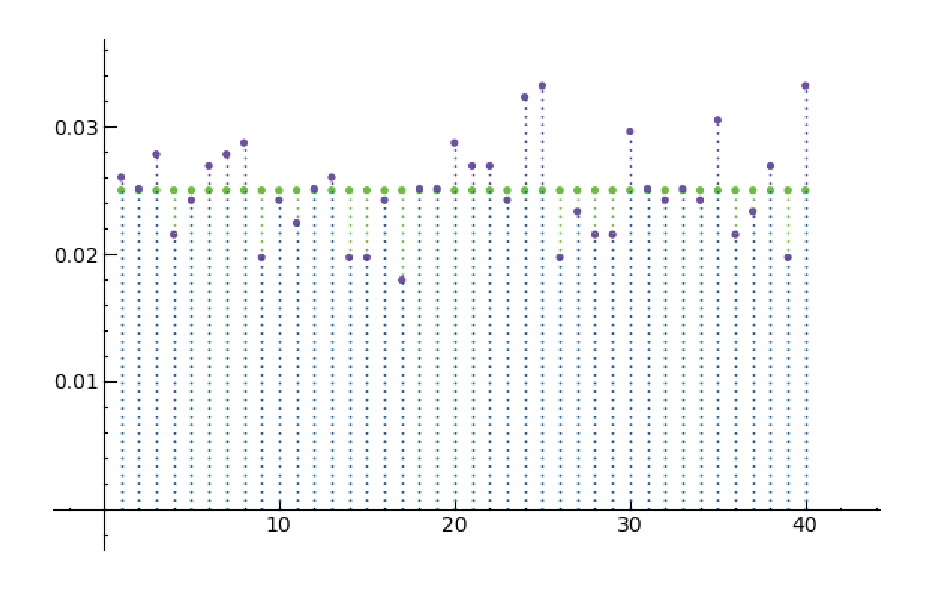
\includegraphics[width=7.5cm,height=4cm]{figures/mylotto_freq_relative}}
\caption{First ball number in 1114 NZ Lotto draws from 1987 to 2008.\label{F:LottoDraws}}
\end{figure}
\end{example}


Next, let us take a detour into how one might interpret it in the real world.  The following is an adaptation from Williams D, {\it Weighing the Odds: A Course in Probability and Statistics}, Cambridge University Press, 2001, which henceforth is abbreviated as WD2001.
\begin{center}
\begin{tabular}{l l}
{\bf Probability Model} & {\bf Real-world Interpretation} \\
Sample space $\Omega$ & Set of all outcomes of an experiment \\
Sample point $\omega$ & Possible outcome of an experiment \\ 
(No counterpart) & Actual outcome $\omega^{\star}$ of an experiment\\
Event A, a (suitable) subset of $\Omega$ & The real-world event corresponding to A \\
 & occurs if and only if $\omega^{\star} \in A$\\
$\p(A)$, a number between $0$ and $1$         & Probability that $A$ will occur for an \\
 & experiment yet to be performed \\
\\
% \end{tabular}
% \end{center}
% \begin{center}
% \begin{tabular}{l l}
{\bf Events in Probability Model} & {\bf Real-world Interpretation} \\
Sample space $\Omega$ & The certain even `something happens' \\
The $\emptyset$ of $\Omega$ & The impossible event `nothing happens' \\ 
The intersection $A \cap B$ & `Both $A$ and $B$ occur'\\
$A_1 \cap A_2 \cap \cdots \cap A_n $ & `All of the events $A_1, A_2, \ldots, A_n$ occur simultaneously'\\
The union $A \cup B$ & `At least one of $A$ and $B$ occurs'\\
$A_1 \cup A_2 \cup \cdots \cup A_n$ & `At least one of the events $A_1, A_2, \ldots, A_n$ occurs'\\
$A^c$, the complement of $A$ & `$A$ does not occur'\\
$A \setminus B$ & `$A$ occurs, but $B$ does not occur'\\
$A \subset B$ & `If $A$ occurs, then $B$ must occur'
\end{tabular}
\end{center}


{In the probability model of Example~\ref{Eg:NZLottoModel}, show that for any event $E \subset \Omega$, \[\p(E)\; =\;
\frac{1}{40} \;\times \;\text{number of elements in $E$} \enspace . \]
}
{\label{Eg:NZLottoExp}}
{
Let $E = \{\omega_1,\omega_2,\ldots,\omega_k\}$ be an event with $k$ outcomes (simple events).  
Then by the addition rule for mutually exclusive events we get:
%\begin{multiline}
$$\p(E)\;=\;\p\left( \{\omega_1,\omega_2,\ldots,\omega_k\} \right)
= \p\left(\bigcup^{k}_{i=1} \{ \omega_i \}\right)\;=\;\sum^{k}_{i=1}\p\left(\{\omega_i\}\right)\;=\;\sum^{k}_{i=1}\frac{1}{40}\;=\;\frac{k}{40} \enspace .$$

%\end{multiline}
}

\subsection{Sigma Algebras of Typical Experiments$^*$}

\begin{example}[`Toss a fair coin once']
Consider the `Toss a fair coin once' experiment.  What is its sample space $\Omega$ and a reasonable collection of events $\C{F}$ that underpin this experiment?  
\[
\Omega = \{  {\tt H}, {\tt T} \}, \qquad \C{F} = \{ {\tt H}, {\tt T},\Omega, \emptyset \} \ ,
\]
A function that will satisfy the definition of probability for this collection of events $\C{F}$ and assign $\p({\tt H}) = \frac{1}{2}$ is summarized below.  First check that the above $\C{F}$ is a sigma-algebra.  Draw a picture for $\p$ with arrows that map elements in the domain $\C{F}$ given above to elements in its range. 
\begin{center}
\begin{tabular*}{3.5in}{@{\extracolsep{\fill}}r c l} \hline
Event $A \in \C{F}$ & $\p : \C{F} \to [0,1]$ & $\p(A) \in [0,1]$ \\ \hline
$\Omega=\{ {\tt H}, {\tt T} \} \, \bullet$ & $ \ \longrightarrow \ $ & $1$ \\ 
${\tt T} \, \bullet$ & $ \ \longrightarrow \ $ & $1-\frac{1}{2}$ \\ 
${\tt H}  \, \bullet$ & $ \ \longrightarrow \ $ & $\frac{1}{2}$ \\ 
$\emptyset \, \bullet$ & $ \ \longrightarrow \ $ & $0$ \\ \hline
\end{tabular*}
\end{center}
\end{example}

\begin{classwork}[The trivial sigma algebra]
Note that $\C{F}' = \{ \Omega, \emptyset\}$ is also a sigma algebra of the sample space $\Omega= \{  {\tt H}, {\tt T} \}$.  Can you think of a probability for the collection $\C{F}'$?
\begin{center}
\begin{tabular*}{3.5in}{@{\extracolsep{\fill}}r c l} \hline
Event $A \in \C{F}'$ & $\p : \C{F}' \to [0,1]$ & $\p(A) \in [0,1]$ \\ \hline
$\Omega=\{ {\tt H}, {\tt T} \} \, \bullet$ & $ \ \longrightarrow \ $ &\\ 
$\emptyset \, \bullet$ & $ \ \longrightarrow \ $ & \\ \hline
\end{tabular*}
\end{center}
{\scriptsize
Thus, $\C{F}$ and $\C{F}'$ are two distinct sigma algebras over our $\Omega=\{ {\tt H}, {\tt T} \}$.  Moreover, $\C{F}' \subset \C{F}$ and is called a sub sigma algebra.  Try to show that $\{\Omega,\emptyset\}$ is the smallest possible sigma algebra over all possible sigma algebras over any given sample space $\Omega$ (think of intersecting an arbitrary family of sigma algebras)?
}
\end{classwork}
 
Generally one encounters four types of sigma algebras (you will understand the last two types after taking more advanced courses in mathematics, so it is fine to understand the ideas intuitively for now!) and they are:
\be
\item
When the sample space $\Omega=\{\omega_1,\omega_2,\ldots,\omega_k\}$ is a finite set with $k$ outcomes and $\p(\omega_i)$, the probability for each outcome $\omega_i \in \Omega$ is known, then one typically takes the sigma-algebra $\C{F}$ to be the set of all subsets of $\Omega$ called the {\bf power set} and denoted by $2^{\Omega}$.  
The probability of each event $A \in 2^{\Omega}$ can be obtained by adding the probabilities of the outcomes in $A$, i.e., $\p(A)=\sum_{\omega_i \in A} \p(\omega_i)$.  
Clearly, $2^{\Omega}$ is indeed a sigma-algebra and it contains $2^{\#\Omega}$ events in it.  

\item
When the sample space $\Omega=\{\omega_1,\omega_2,\ldots\}$ is a countable set then one typically takes the sigma-algebra $\C{F}$ to be the set of all subsets of $\Omega$.  Note that this is very similar to the case with finite $\Omega$ except now $\C{F}=2^{\Omega}$ could have uncountably many events in it.

%%TODO make an example of a continuous space experiment, say Darth Mole's light saber for R^1 and destination of a random ride in Doctor Who's TARDIS space-time R^d 
\item
If $\Omega = \Rz^d$ for finite $d \in \{1,2,3,\ldots\}$ then the {\bf Borel sigma-algebra} is the smallest sigma-algebra containing 
all {\bf half-spaces}, i.e., sets of the form 
$$\{x=(x_1,x_2,\ldots,x_d) \in \Rz^d: x_1 \leq c_1, x_2 \leq c_2, \ldots, x_d \leq c_d\}, \quad \text{ for any } c=(c_1,c_2,\ldots,c_d)\in\Rz^d \enspace ,
$$
When $d=1$ the half-spaces are the half-lines $\{(-\infty,c]: c \in \Rz\}$ and when $d=2$ the half-spaces are the south-west quadrants $\{(-\infty,c_1]\times(-\infty,c_2] : (c_1,c_2) \in \Rz^2\}$, etc.  
(Equivalently, the Borel sigma-algebra is the smallest sigma-algebra containing all open sets in $\Rz^d$). 

\item
Given a finite set $\Sz=\{s_1,s_2,\ldots,s_k\}$, let $\Omega$ be the sequence space $\Sz^{\infty}:=\Sz \times \Sz \times \Sz \times\cdots$, i.e., the set of sequences of infinite length that are made up of elements from $\Sz$.  
A set of the form
\[
A_1 \times A_2 \times \cdots \times A_n \times \Sz \times \Sz \times \cdots, \quad A_k \subset \Sz \text{ for all } k \in \{1,2,\ldots,n\} \enspace ,
\]
is called a {\bf cylinder set}.  
The set of events in $\Sz^{\infty}$ is the smallest sigma-algebra containing the cylinder sets. 

\begin{itemize}
\item {\bf A most primitive sigma-algebra for probability theory:} 
For example if $\Sz=\{0,1\}$, then $\Omega = \{0,1\}^{\infty}$ is the set of all infinite sequences made of $0$'s and $1$'s. 
To take advantage of arithmetic and analysis, $\Omega$ can be seen as the binary representation of all real numbers in the unit interval $[0,1]$.  
We can take advantage of combinatorics and algebra if we further represent the dyadic partition of $[0,1]$ by a binary tree (as drawn in lectures). 
Then, a cylinder set such as $1 \times 1 \times 0 \times \{0,1\} \times \{0,1\} \times \cdots$, an event here, can be interpreted as the finite binary sequence $(1,1,0)$ --- corresponding to the third leaf of a finite binary tree with four leaves obtained by splitting the right-most leaf twice. This cylindrical event $(1,1,0)$ contains all real numbers in the interval $[\frac{3}{4},\frac{7}{8}] \subset [0,1] =: \Omega$.\end{itemize}

\ee

\begin{Exercise}[title={intuiting sigma-algebra -- this is optional},label={underMPSA}]
Try to carefully recollect and understand the most primitive sigma-algebra in the last item above as it was explained in lectures.
%\ExePart
%\Question
%\subQuestion Show that...
%\subQuestion In this question...
%\subsubQuestion Show that...
%\subsubQuestion Conclude...
%\subQuestion Conclude.
%\Question Show that if $b > 1$...
%\ExePart
%\Question What happens to if $b=1$?
\end{Exercise}
\begin{Answer}
This is an optional exercise. You will understand this as you progress through your mathematics programme. 
The explanation in the said item was (or will be explained in person again) in the lectures. 
This exercise was created to answer natural questions that were asked by students who wanted to know.
\end{Answer}


\begin{framed}
PROBABILITY SUMMARY

\medskip

Axioms:
\begin{enumerate}
\item If $A\subseteq \Omega$ then $0\leq \p(A)\leq 1$ and $\p(\Omega)=1$.
\item If $A$, $B$ are disjoint events, then $\p(A\cup B)=\p(A)+\p(B)$.

[This is true only when $A$ and $B$ are disjoint.]
\item If $A_1,A_2,\dots$ are disjoint then $\p(A_1\cup A_2
\cup\dots)=\p(A_1)+\p(A_2)+\dots$
\end{enumerate}
Rules:
$$\p(A^c)\;=\;1-\p(A)$$
$$\p(A\cup B)\;=\;\p(A)+\p(B)-\p(A\cap B) \qquad [\textrm{always true}]$$
\end{framed}

\section{Exercises in Probability}\label{S:xsProbability}

\begin{ExerciseList}
\Exercise
{In English language text, the twenty six letters in the alphabet occur with the following frequencies:
{\footnotesize $$
\mathsf{
\begin{array}{cccccccccccccccccc}
\sf E   &       13      \%&     \sf R   &       7.7     \%&     \sf A   &       7.3     \%&     \sf H   &       3.5     \%&     \sf F   &       2.8     \%&     \sf M    &      2.5     \%&     \sf W   &       1.6     \%&     \sf X   &       0.5     \%&     \sf J   &       0.2     \%\\
\sf T   &       9.3     \%&     \sf O   &       7.4     \%&     \sf S   &       6.3     \%&     \sf L   &       3.5     \%&     \sf P   &       2.7     \%&     \sf Y    &      1.9     \%&     \sf V   &       1.3     \%&     \sf K   &       0.3     \%&     \sf Z   &       0.1     \%\\
\sf N   &       7.8     \%&     \sf I   &       7.4     \%&     \sf D   &       4.4     \%&     \sf C   &       3       \%&     \sf U   &       2.7     \%&     \sf G    &      1.6     \%&     \sf B   &       0.9     \%&     \sf Q   &       0.3     \%&             &               \\
\end{array}
}
$$}
Suppose you pick one letter at random from a randomly chosen English
book from our central library with
$\Omega=\{\mathsf{A,B,C,\ldots,Z}\}$ (ignoring upper/lower cases),
then what is the probability of these events?
\begin{itemize}
\item[(a)]$\p(\{\mathsf{Z}\})$
\item[(b)]$\p(\textrm{`picking any letter'})$
\item[(c)] $\p(\{\mathsf{E},\mathsf{Z}\})$
\item[(d)]$\p(\textrm{`picking a vowel'})$
\item[(e)]$\p(\textrm{`picking any letter in the word WAZZZUP'})$
\item[(f)]$\p(\textrm{`picking any letter in the word WAZZZUP or a vowel'})$.
\end{itemize}
}
\label{Ex:RandomEnglishLetter}
\Answer
{\bit
\item[(a)] $\p(\{\mathsf{Z}\})=0.1\%=\frac{0.1}{100}=0.001$
\item[(b)] $\p(\textrm{`picking any letter'})= \p(\Omega) = 1$
\item[(c)] $\p(\{\mathsf{E},\mathsf{Z}\}) =\p(\{\mathsf{E}\} \cup
    \{\mathsf{Z}\} ) =  \p(\{\mathsf{E}\})+\p(\{\mathsf{Z}\}) =
    0.13+0.001=0.131$, by Axiom~(3)
\item[(d)] $\p(\textrm{`picking a
    vowel'})=\p(\{\mathsf{A,E,I,O,U}\})=(7.3\%+13.0\%+7.4\%+7.4\%+2.7\%)=37.8\%$,  by the addition rule for mutually exclusive events, rule (2).
\item[(e)] $\p(\textrm{`picking any letter in the word
    WAZZZUP'})=\p(\{\mathsf{W,A,Z,U,P}\})=14.4\%$,  by the
  addition rule for mutually exclusive events, rule (2).
\item[(f)] $\p(\textrm{`picking any letter in the word WAZZZUP or a vowel'})=$\\
$\p(\{\mathsf{W,A,Z,U,P}\})+\p(\{\mathsf{A,E,I,O,U}\})-\p(\{\mathsf{A,U}\})
  = 14.4\% + 37.8\% - 10\% = 42.2\%$,  by the addition rule for two
arbitrary events, rule (3).
\eit
}


\Exercise
Find the sample spaces  for the following experiments:
\begin{enumerate}
\item Tossing 2 coins whose faces are sprayed with black paint denoted by $\mathsf{B}$ and white paint denoted by $\mathsf{W}$.
\item Drawing 4 screws from a bucket  of left-handed and right-handed screws
  denoted by $\mathsf{L}$ and $\mathsf{R}$, respectively.
\item Rolling a die and recording the number on the upturned face  until the first $\mathsf{6}$ appears.
\end{enumerate}
\Answer
\be
\item $\{\mathsf{BB},\mathsf{BW},\mathsf{WB},\mathsf{WW}\}$

\item $\begin{aligned}\{\mathsf{ RRRR,RRRL,RRLR,RLRR,LRRR,RLRL,RRLL,LLRR,}
    \\ \mathsf{LRLR,LRRL,RLLR,LLLL, LLLR,LLRL,LRLL,RLLL}\}\end{aligned}$
\item $\{6,16,26,36,46,56,116, 126,136, 146, 156,
      216, 226, 236, 246, 256, \,\ldots\}$
\ee


\Exercise
Suppose we pick a letter at random from the word WAIMAKARIRI. 
\begin{enumerate}
\item What is the sample space $\Omega$?
\item  What probabilities should be assigned to the outcomes?
\item What is the probability of {\emph not} choosing the letter  R?
\end{enumerate}
\Answer

\be
\item The sample space $\Omega=\{\mathsf{W},\mathsf{A},\mathsf{I},\mathsf{M},\mathsf{K},\mathsf{R}\}$.
\item   Since there are eleven letters in WAIMAKARIRI the probabilities are:
\cen{ $\p(\sf\{W\})=\frac{1}{11}$, $\p(\sf\{ A\})=\frac{3}{11}$, $\p( \sf\{ I\})
=\frac{3}{11}$,
    $\p(\sf\{ M\})=\frac{1}{11}$, $\p(\sf\{ K\})=\frac{1}{11}$, $\p(\sf\{
    R\})=\frac{2}{11}$\,.}

\item By the complementation rule, the probability of not choosing
    the letter R is:  \[1\,-\,\p(\text{choosing the letter R})\,=\,1\,-\, \frac{2}{11}\,=\,\frac{9}{11}\,.\]

\ee


\Exercise
There are seventy five balls in total inside the Bingo Machine.  
Each ball is labelled by one of the following five letters: 
$\mathsf{B}$, $\mathsf{I}$, $\mathsf{N}$, $\mathsf{G}$, and $\mathsf{O}$.  
There are fifteen balls labelled by each letter.  
The letter on the first ball that comes out of a BINGO machine after it has been well-mixed is the outcome of our experiment. 
\begin{itemize}
\item[(a)] Write down the sample space of this experiment.
\item[(b)] Find the probabilities of each simple event.
\item[(c)] Show that $\p(\Omega)$ is indeed $1$.
\item[(d)] Check that the addition rule for mutually exclusive events holds for the simple events $\{B\}$ and $\{I\}$. 
\item[(e)]Consider the following events: 
$C = \{\mathsf{B},\mathsf{I},\mathsf{G}\}$ and $D = \{\mathsf{G},\mathsf{I},\mathsf{N}\}$.  
Using the addition rule for two arbitrary events, find  $\p(C \cup D)$.
\end{itemize}

\Answer
\be
\item
First, the sample space is: $\Omega=\{ {\mathsf{B}, \mathsf{I},
  \mathsf{N}, \mathsf{G}, \mathsf{O} } \} \enspace . $
\medskip

\item The probabilities of simple events are:
$$
\p(\mathsf{B} )\;=\;\p(\mathsf{I})\;=\;\p(\mathsf{N})\;=\;\p(\mathsf{G})\;=\;\p(\mathsf{O})\;=\;{\frac{15}{75}\;=\;\frac{1}{5}} \enspace .
$$

\item 

%Axiom~(1):
%$${0\leq \p(\mathsf{B})\;=\;\p(\mathsf{I})\;=\;\p(\mathsf{N})\;=\;\p(\mathsf{G})\;=\;\p(\mathsf{O})\;=\;\frac{1}{5} \leq 1 \enspace .}
%$$

%Axiom~(2): 
Using the addition rule for mutually exclusive events,
\begin{eqnarray*}
\p(\Omega)
&=& \p(\mathsf{\{B,I,N,G,O\}})\\
&=& \p(\{\sf{B}\} \cup\{\sf{I}\}\cup \{\sf{N}\} \cup \{\sf{G}\} \cup \{\sf{O}\})\\
&=& \p(\sf B)+\p(\sf I)+\p(\sf N)+\p(\sf G)+\p(\sf O) \quad \text{simplifying notation} \\
&=& \frac{1}{5}+\frac{1}{5}+\frac{1}{5}+\frac{1}{5}+\frac{1}{5}\\
&=& 1
\end{eqnarray*}

\item Since the   events $\{\sf B\}$ and $\{\sf I\}$ are disjoint,
$$
\p(\{\sf{B}\} \cup \{\sf{I}\})\;=\;\p(\sf B)+\p(\sf I)\;=\;\frac{1}{5}+\frac{1}{5}\;=\;\frac{2}{5}\,.
$$


\medskip


\item  Using the addition rule for two arbitrary events we get,
\begin{eqnarray*}
\p(C \cup D) &=& \p(C)+\p(D)-\p(C\cap D)\\& =& \p(\{\sf{B},\sf{I},\sf{G}\}) + \p(\{\sf{G},\sf{I},\sf{N}\}) - \p(\{\sf{G},\sf{I}\})\\
& =& \frac{3}{5} +\frac{3}{5} - \frac{2}{5}\\& = &\frac{4}{5} \enspace .
\end{eqnarray*}
\ee


\end{ExerciseList}



\section{Conditional Probability}\label{S:CondProb}
Next, we define conditional probability and the notion of independence of events.  We use the LTRF idea to motivate the definition.
\begin{idea}[LTRF intuition for conditional probability]
Let $A$ and $B$ be any two events associated with our experiment $\E{E}$ with $\p(A) \neq 0$.  The `conditional probability that $B$ occurs given that $A$ occurs' denoted by $\p(B|A)$ is again intuitively underpinned by the super-experiment $\E{E}^{\infty}$ which is the `independent' repitition of our original experiment $\E{E}$ `infinitely' often.  The LTRF idea is that $\p(B|A)$ is the long-term proportion of those experiments on which $A$ occurs that $B$ also occurs.
 
Recall that $N(A,n)$ as defined in \eqref{E:NofAn} is the fraction of times $A$ occurs out of $n$ independent repetitions of our experiment $\E{E}$ (ie.~the experiment $\E{E}^{n}$).  If $A \cap B$ is the event that `$A$ and $B$ occur simultaneously', then we intuitively want
\[
\p(B|A) \quad \lq\lq \rightarrow " \quad \frac{N(A \cap B,n)}{N(A,n)} = \frac{N(A \cap B,n)/n}{N(A,n)/n} =  \frac{\p(A \cap B)}{\p(A)}
\]
as our $\E{E}^{n} \rightarrow \E{E}^{\infty}$.  So, we {\bf define} conditional probability as we want.
 \end{idea}
 \begin{definition}[Conditional Probability]\label{D:CondProb}
Suppose we are given an experiment $\E{E}$ with a triple $(\Omega, \C{F}, \p)$.  Let $A$ and $B$ be events, ie.~$A,B \in \C{F}$, such that $\p(A) \neq 0$.  Then, we define the {\bf conditional probability} of $B$ given $A$ by,
 \begin{equation}\label{E:CPD}
 \p(B|A) := \frac{\p(A \cap B)}{\p(A)} \ .
 \end{equation}
 Note that for a {\bf fixed} event $A \in \C{F}$ with $\p(A)>0$ and {\bf any} event $B \in \C{F}$, the conditional  probability $\p(B | A)$ is a probability as in \hyperref[D:Prob]{Definition \ref*{D:Prob}}, ie.~a function:
 \[
 \p(B | A) : \C{F} \rightarrow [0,1]
 \]
 that assigns to each $B \in \C{F}$ a number in the interval $[0,1]$, such that,
 \begin{enumerate}
 \item $\p(\Omega | A) = 1$ \qquad Meaning `Something Happens given the event A happens'
 \item The `Addition Rule' axiom holds, ie.~for events $B_1, B_2 \in \C{F}$,
 \[
 B_1 \cap B_2 = \emptyset \quad \text{implies} \quad \p(B_1 \cup B_2 | A) = \p(B_1 | A) + \p(B_2 |  A)  \ .
 \]

\item For mutually exclusive or pairwise-disjoint events, $B_1,B_2, \ldots$,
\[
\p(B_1 \cup B_2 \cup \cdots | A) = \p(B_1|A)+\p(B_2|A)+\cdots \enspace .
\]
\end{enumerate} 
\end{definition}

From the definition of conditional probability we get the following rules:
\be
\item Complementation rule: $\p(B | A)\, = \,1 - \p(B^c | A)$ .

\item Addition rule for two arbitrary events $B_1$ and $B_2$: \[{\p(B_1 \cup B_2 | A) \;= \;\p(B_1 | A) + \p(B_2 | A) - \p(B_1\cap B_2|A)}\,.\]

\item Multiplication rule for two likely events: 

If $A$ and $B$ are events, and if
  $\p(A)\neq 0$ and  $\p(B)\neq 0$, then
\[\p(A\cap B)\;=\;\p(A)\p(B|A)\;=\;\p(B)\p(A|B)\,. \]
\ee

\begin{example}[Wasserman03, p.~11]
 A medical test for a disease $D$ has outcomes $+$ and $-$.  the probabilities are:
\begin{center}
 \begin{tabular}{l | c | c}
 \hline
 & Have Disease ($D$) & Don't have disease ($D^c$)  \\ \hline
Test positive ($+$) & 0.009 & 0.099 \\
 Test negative ($-$) & 0.001 & 0.891\\ \hline
 \end{tabular}
 \end{center}
 Using the definition of conditional probability, we can compute the conditional probability that you test positive given that you have the disease:
 \[
 \p(+ | D) = \frac{\p(+ \cap D)}{\p(D)} = \frac{0.009}{0.009+0.001}=0.9 \ ,
 \]
 and the conditional probability that you test negative given that you don't have the disease:
 \[
 \p(- | D^c) = \frac{\p(- \cap D^c)}{\p(D^c)} = \frac{0.891}{0.099+0.891} \approxeq 0.9 \ .
 \]
 Thus, the test is quite accurate since sick people test positive 90\% of the time and healthy people test negative 90\% of the time.
 
Now, suppose you go for a test and and test positive.  What is the probability that you have the disease ?
 \[
 \p(D|+) = \frac{\p(D \cap +)}{\p(+)} = \frac{0.009}{0.009+0.099} \approxeq 0.08
 \]
Most people who are not used to the definition of conditional probability would intuitively associate a number much bigger than $0.08$ for the answer.  Interpret conditional probability in terms of the meaning of the numbers that appear in the numerator and denominator of the above calculations.
\end{example}
 
 Next we look at one of the most elegant applications of the definition of conditional probability along with the addition rule for a partition of $\Omega$.
 \begin{prop}[Bayes' Theorem, 1763]
 Suppose the events $A_1,A_2,\ldots,A_k \in \C{F}$, with $\p(A_h)>0$ for each $h \in \{1,2,\ldots,k\}$, partition the sample space $\Omega$, ie.~they are mutually exclusive (disjoint) and exhaustive events with positive probability: 
 \[
 A_i \cap A_j = \emptyset, \ \text{for any distinct $i,j \in \{1,2,\ldots,k\}$}, \qquad \bigcup_{h=1}^k A_h = \Omega, \qquad \p(A_h) > 0
 \]
 Thus, precisely one of the $A_h$'s will occur on any performance of our experiment $\E{E}$.  
 
 Let $B \in \C{F}$ be some event with $\p(B) > 0$, then 
 \begin{equation}\label{E:BayesThm}
 \p(A_h|B) = \frac{\p(B|A_h) \p(A_h)}{\sum_{h=1}^k \p(B|A_h) \p(A_h)}
 \end{equation}
 {\scriptsize
 \begin{proof}
 We apply elementary set theory, the definition of conditional probability $k+2$ times and the addition rule once:
 \begin{eqnarray}
 \p(A_h | B) &=& \frac{\p(A_h \cap B)}{\p(B)} = \frac{\p( B \cap A_h)}{\p(B)} = 
 \frac{\p( B | A_h) \p(A_h)}{\p(B)}  \notag \\
 &=& \frac{\p( B | A_h) \p(A_h)}{\p \left( \bigcup_{h=1}^k (B \cap A_h) \right)} =
 \frac{\p( B | A_h) \p(A_h)}{\sum_{h=1}^k \p \left( B \cap A_h \right)} \notag \\
 &=& \frac{\p( B | A_h) \p(A_h)}{\sum_{h=1}^k \p(B | A_h) \p(A_h)} \notag
 \end{eqnarray}
 \end{proof}
}
The operations done to the denominator in the proof above:
\begin{equation}\label{E:LTP}
\p( B) = \sum_{h=1}^k \p(B | A_h) \p(A_h)
\end{equation}
is also called `the law of total probability' or `the total probability theorem'.  
We call $\p(A_h)$ the {\bf prior probability of} $A_h$ and $\p(A_h|B)$ the {\bf posterior probability of} $A_h$.
 \end{prop}

\begin{example}[Wasserman2003~p.12]
Suppose Larry divides his email into three categories: $A_1 = \text{``spam''}$, $A_2 =\text{ ``low priority''}$, and $A_3 = \text{ ``high priority''}$.  From previous experience, he finds that $\p(A_1) = 0.7$, $\p(A_2) = 0.2$ and $\p(A_3)=0.1$.  Note that $\p(A_1 \cup A_2 \cup A_3) = \p(\Omega) = 0.7+0.2+0.1 = 1$.  Let $B$ be the event that the email contains the word ``free.''  From previous experience, $\p(B|A_1) = 0.9$, $\p(B|A_2) = 0.01$ and $\p(B|A_3)=0.01$.  Note that $\p(B|A_1) + \p(B|A_2) + \p(B|A_3) = 0.9+0.01+0.01 \neq 1$.  Now, suppose Larry receives an email with the word ``free.''  What is the probability that it is ``spam,'' ``low priority,''  and ``high priority'' ?
%{\color{Gray}{

{\scriptsize{
\[
\begin{array}{l l l l l}
\p(A_1 | B) 
&= \frac{\p(B|A_1)\p(A_1)}{\p(B|A_1)\p(A_1)+\p(B|A_2)\p(A_2)+\p(B|A_3)\p(A_3)} 
&= \frac{0.9 \times 0.7}{(0.9 \times 0.7)+ (0.01 \times 0.2) + (0.01 \times 0.1)}
&= \frac{0.63}{0.633}
&\approxeq 0.995 \\
\\
\p(A_2 | B) 
&= \frac{\p(B|A_2)\p(A_2)}{\p(B|A_1)\p(A_1)+\p(B|A_2)\p(A_2)+\p(B|A_3)\p(A_3)} 
&= \frac{0.01 \times 0.2}{(0.9 \times 0.7)+ (0.01 \times 0.2) + (0.01 \times 0.1)}
&= \frac{0.002}{0.633}
&\approxeq 0.003 \\
\\
\p(A_3 | B) 
&= \frac{\p(B|A_3)\p(A_3)}{\p(B|A_1)\p(A_1)+\p(B|A_2)\p(A_2)+\p(B|A_3)\p(A_3)} 
&= \frac{0.01 \times 0.1}{(0.9 \times 0.7)+ (0.01 \times 0.2) + (0.01 \times 0.1)}
&= \frac{0.001}{0.633}
&\approxeq 0.002 \\
\end{array}
\]
Note that $\p(A_1|B) + \p(A_2|B)+\p(A_3|B) = 0.995+0.003+0.002=1$.
}}
%}}
\end{example}

\begin{example}[Urn with red and black balls] 
A well-mixed urn contains five
{\sf red} and ten {\sf black} balls. We draw two balls from the urn
without replacement. What is the probability that the second ball drawn
is {\sf red}?

This is easy to see if we draw a probability tree diagram.  
The first split in the tree is based on the outcome of the first draw and the second on the outcome of the last draw.  
The outcome of the first draw dictates the probabilities for the second one since we are sampling without replacement.  
We multiply the probabilities on the edges to get probabilities of the four endpoints, and then sum the ones that correspond to {\sf red} in the second draw, that is
\[
P(\text{second ball is red}) \;=\; 4/42+10/42\;=\;1/3 \enspace .
\]

\begin{center}
\begin{picture}(100,140)(75,30)
\drawline(0,90)(75,120)(125,140)
\drawline(75,120)(125,100)
\drawline(0,90)(75,60)(125,40)
\drawline(75,60)(125,80)
\put(55,125){{\sf red}}\put(55,45){{\sf black}}
\put(130,140){$\mathsf{(red, red)}$ 4/42}\put(130,100){$\mathsf{(red, black)}$ 10/42}
\put(130,80){$\mathsf{(black, red)}$ 10/42}\put(130,40){$\mathsf{(black, black)}$ 18/42}
\put(95,140){4/14}\put(95,115){10/14}
\put(95,80){5/14}\put(95,55){9/14}
\put(30,110){1/3}\put(30,80){2/3}
\end{picture}
\end{center}

Alternatively,  use the total probability theorem to break
the problem  down into manageable pieces.  
Let
  $R_1=\{\mathsf{(red,red),(red,black)}\}$ and
  $R_2=\{\mathsf{(red,red),(black,red)}\}$ be the events corresponding
  to a {\sf red} ball in the $1$st and $2$nd draws, respectively, and
  let $B_1=\{\mathsf{(black,red),(black,black)}\}$ be the event of a
  {\sf black} ball on the first draw.

Now $R_1$ and $B_1$ partition $\Omega$ so we can  write:
\begin{eqnarray*}
P(R_2)
&=& \p(R_2\cap R_1) + \p(R_2\cap B_1)\\[6pt]
&=& \p\;(R_2| R_1)\p(R_1) + \p(R_2|B_1)\p(B_1)\\[6pt]
&=& (4/14)(1/3)\,+\,(5/14)(2/3) =  1/3 \enspace .
\end{eqnarray*}
\end{example}

 \subsection{Independence and Dependence}\label{S:IndepDep}
 \begin{definition}[Independence of two events]\label{D:IndOf2Events}
 Any two events $A$ and $B$ are said to be {\bf independent} if and only if
 \begin{equation}\label{E:PofAB=PAPB}
 \p(A \cap B) = \p(A) \p(B) \ .
 \end{equation}
 \end{definition}
 Let us make sense of this definition in terms of our previous definitions.  When $\p(A)=0$ or $\p(B)=0$, both sides of the above equality are $0$.  If $\p(A) \neq 0$, then rearranging the above equation we get:
 \[
 \frac{\p(A \cap B)}{\p(A)} = \p(B) \ .
 \]
 But, the LHS is $\p(B|A)$ by \hyperref[E:CPD]{definition \ref*{E:CPD}}, and thus for independent events $A$ and $B$, we get:
 \[
 \p(B|A) = \p(B) \ .
 \]
This says that information about the occurrence of $A$ does not affect the occurrence of $B$.  If $\p(B) \neq 0$, then an analogous argument:
{\scriptsize
\[
\p(A \cap B) = \p(A) \p(B) \iff \p(B \cap A) = \p(A) \p(B) \iff \frac{\p(B \cap A)}{\p(B)} = \p(A) \iff  \p(A|B) = \p(A) \ ,
\]
}
says that information about the occurrence of $B$ does not affect the occurrence of $A$.  Therefore, the probability of their joint occurence $\p(A \cap B)$ is simply the product of their individual probabilities $\p(A) \p(B)$.

\begin{definition}[Independence of a sequence of events]\label{D:IndOfSeqOfEvents}
We say that a finite or infinite sequence of events $A_1,A_2,\ldots$ are independent if whenever $i_1,i_2,\ldots,i_k$ are distinct elements from the set of indices $\Nz$, such that $A_{i_1},A_{i_2},\ldots,A_{i_k}$ are defined (elements of $\C{F}$), then
\[
\p(A_{i_1} \cap A_{i_2} \ldots \cap A_{i_k})  =  \p(A_{i_1} ) \p(A_{i_2})  \cdots \p(A_{i_k}) 
\]
\end{definition}

\begin{example}[Some Standard Examples]
A sequence of events in a sequence of independent trials is independent.
\be

\item[(a)] Suppose you toss a fair coin twice such that the first toss is independent of the second.  Then,
$$
\p(\mathsf{Heads} \text{ on the first toss} \cap \mathsf{Tails} \text{ on the second toss} ) = \p(\mathsf{H}) \p(\mathsf{T}) = \frac{1}{2} \times \frac{1}{2}= \frac{1}{4} \enspace .
$$

\item[(b)] Suppose you independently toss a fair die three times.  Let $E_i$ be the event that the outcome is an even number on the $i$-th trial.  The probability of getting an even number in all three trials is:
\begin{eqnarray*}
\p(E_1 \cap E_2 \cap E_3)
&=& \p(E_1) \p(E_2) \p(E_3)\\
&=& \left(\p(\{\mathsf{2,4,6}\})\right)^3\\
&=& \left(\p(\{\mathsf{2}\} \cup \{\mathsf{4}\} \cup \{\mathsf{6}\}) \right)^3 \\
&=& \left(\p(\{\mathsf{2}\}) + \p(\{\mathsf{4}\}) + \p(\{\mathsf{6}\})\right)^3\\
&=& \left(\frac{1}{6} + \frac{1}{6} + \frac{1}{6} \right)^3 
= \left(\frac{1}{2} \right)^3
= \frac{1}{8} \enspace .
\end{eqnarray*}
%This is an obvious answer but there is a lot of maths going on here!

\item[(c)]Suppose you toss a fair coin independently $m$ times.  Then each of the $2^m$ possible outcomes in the sample space $\Omega$ has equal probability of $\frac{1}{2^m}$ due to independence.
\ee
\end{example}

\begin{example}[dependence and independence] 
Suppose we toss two fair dice.  
Let $A$ denote the event that the sum of the dice is six and $B$ denote the event that the first die equals four.  The sample space encoding the thirty six ordered pairs of outcomes for the two dice is $\Omega = \{ (1,1), (1,2), \ldots, (1,6), (2,1), \ldots, (2,6), \ldots, (5,6), (6,6)\}$ and due to independence $\p(\omega)=1/36$ for each $\omega\in\Omega$.  
Then 
\[
\p(A \cap B)  = \p (\{(4,2)\}) = \frac{1}{36} \enspace ,
\]
but
\begin{eqnarray*}
\p(A)\p(B) 
&=& \p (\{(1,5),(2,4),(3,3),(4,2),(5,1)\}) \p( \{ (4,1),(4,2),(4,3),(4,4),(4,5),(4,6) \}) \\
&=& \frac{5}{36}\times \frac{6}{36} = \frac{5}{36}\times\frac{1}{6} = \frac{5}{216} \enspace ,
\end{eqnarray*}
and therefore $A$ and $B$ are not independent.  
The reason for the events $A$ and $B$ being dependent is clear because the chance of getting a total of six depends on the outcome of the first die (not being six).

Now, let $C$ be the event that the sum of the two dice equals seven.  
Then
\[
\p(C \cap B)  = \p (\{(4,3)\}) = \frac{1}{36} \enspace ,
\]
while
\begin{eqnarray*}
\p(C \cap B)  
&=& \p (\{(1,6),(2,5),(3,4),(4,3),(5,2),(6,1)\}) \p( \{ (4,1),(4,2),(4,3),(4,4),(4,5),(4,6) \})\\
&=& \frac{6}{36}\times\frac{6}{36}= \frac{1}{36} \enspace ,
\end{eqnarray*}
and therefore $C$ and $B$ are independent events.  Once again this is clear because the chance of getting a total of seven does not depend any more on the outcome of the first die (it is allowed to be any one of the six possible outcomes). 
\end{example}

\begin{example}[Pairwise independent events that are not jointly independent]
Let a ball be drawn from an well-stirred urn containing four balls labelled 1,2,3,4.  
Consider the events $A = \{1,2\}$, $B=\{1,3\}$ and $C=\{1,4\}$.  
Then,
\begin{eqnarray*}
\p(A \cap B) &=& \p(A)\p(B) = \frac{2}{4}\times\frac{2}{4} = \frac{1}{4},\\
\p(A \cap C) &=& \p(A)\p(C) = \frac{2}{4}\times\frac{2}{4} = \frac{1}{4},\\
\p(B \cap C) &=& \p(B)\p(C) = \frac{2}{4}\times\frac{2}{4} = \frac{1}{4},
\end{eqnarray*}
but,
\[
\frac{1}{4} = \p(\{1\}) = \p (A \cap B \cap C) \neq \p(A)\p(B)\p(C) = \frac{2}{4}\times\frac{2}{4}\times\frac{2}{4}=\frac{1}{8} \enspace .
\]
Therefore, inspite of being pairwise independent, the events $A$, $B$ and $C$ are not jointly independent.
\end{example}

\section*{Exercises}

\begin{ExerciseList}

\Exercise
What gives the greater probability of hitting some target at least
  once: 
\begin{enumerate}
\item  hitting in a shot with probability $\frac{1}{2}$ and firing 1 shot, or 
\item hitting in a shot with probability $\frac{1}{3}$ and firing 2 shots?
\end{enumerate}
First guess. Then calculate.

\Answer
We can assume  that the first shot is independent of
the second shot so we can multiply the probabilities here.

For case A, there is only one shot so the probability of hitting at least once is $\frac{1}{2}$.

For case B, the probability of missing both shots is
$\frac{2}{3}\,\frac{2}{3}\,=\,\frac{4}{9}$,  so  the probability hitting some target at least once is
  \[ 1- \p(\text{missing the target both times})\;=\; 1-\frac{4}{9}\;=\;\frac{5}{9}\]
Therefore, case B has the greater probability of hitting the target at least once.

\Exercise
Suppose we independently roll two fair dice each of whose faces are marked by numbers
  $\sf 1$,$\sf 2$,$\sf 3$,$\sf 4$, $\sf 5$ and $\sf 6$.
\begin{enumerate}
\item List the sample space for the experiment if we note the   numbers
  on the 2 upturned faces.
\item What is the probability of obtaining a sum greater than 4 but less
  than 7?
\end{enumerate}

\Answer
\be
\item The sample space is
$$
\begin{aligned}
\{
\mathsf{(1,1),(1,2),(1,3),(1,4),(1,5),(1,6),\quad (2,1),(2,2),(2,3),(2,4),(2,5),(2,6),}\\
\mathsf{(3,1),(3,2),(3,3),(3,4),(3,5),(3,6),\quad (4,1),(4,2),(4,3),(4,4),(4,5),(4,6),}\\
\mathsf{(5,1),(5,2),(5,3),(5,4),(5,5),(5,6),\quad (6,1),(6,2),(6,3),(6,4),(6,5),(6,6)}
\}
\end{aligned}
$$
Note: Order matters here. For example, the outcome ``16'' refers to a ``1'' on the first die and a ``6'' on the second,
whereas the outcome ``61'' refers to a ``6'' on the first die and a ``1'' on the
second.

\item First tabulate all possible sums as follows:
$$
\begin{array}{c|cccccc}
+       &       1       &       2       &       3       &       4       &       5       &       6       \\\hline
1       &       2       &       3       &       4       &       \mathbf{5}      &       \mathbf{6}      &       7       \\
2       &       3       &       4       &       \mathbf{5}      &       \mathbf{6}      &       7       &       8       \\
3       &       4       &       \mathbf{5}      &       \mathbf{6}      &       7       &       8       &       9       \\
4       &       \mathbf{5}      &       \mathbf{6}      &       7       &       8       &       9       &       10      \\
5       &       \mathbf{6}      &       7       &       8       &       9       &       10      &       11      \\
6       &       7       &       8       &       9       &       10      &       11      &       12      \\
\end{array}$$
 Let $A$ be the event {\em the sum is 5} and $B$ be the event {\em
    the sum is 6}, then $A$ and $B$ are mutually exclusive events with
  probabilities \[\p(A) = \frac{4}{36} \quad \text{and}\quad \p(B) =
  \frac{5}{36} \,.\]
Therefore,
   $$\p(4<\textrm{sum }<7)\;=\; \p( A \cup B) \;=\; \p(A)\,+\,\p(B)\;=\; \frac{4}{36} +
\frac{5}{36} \;=\;\frac{1}{4}$$
\ee


\Exercise
Based on past experience, 70\% of students in a certain course pass the midterm test.  
The final exam is passed by 80\% of those who passed the midterm test, but only by 40\% of those who fail the midterm test.  
What fraction of students pass the final exam?

\Answer
First draw a tree  with the first split based on the outcome of the midterm test and the second on the outcome of the final exam.  
Note that the probabilities involved in this second branch are {\em conditional} probabilities that depend on the outcome of the midterm test.  
Let $A$ be the event that the student passes the final exam and let $B$ be the event that the student passes the midterm test.

\begin{center}
\begin{picture}(100,160)(75,30){\drawline(0,90)(75,120)(125,140)
\drawline(75,120)(125,100)\drawline(0,90)(75,60)(125,40)
\drawline(75,60)(125,80)
\put(55,125){$B$}\put(55,50){$B^c$}
\put(130,140){$A$\quad $\p(A \cap  B) = 0.56$}\put(130,100){$A^c$ \quad
  $\p(A^c\cap B)= 0.14$}
\put(130,80){$A$ \quad $\p(A\cap B^c) = 0.12$ }\put(130,40){$A^c$ \quad
  $\p(A^c\cap B^c)= 0.18$}
\put(100,137){0.8}\put(100,112){0.2}
\put(100,77){0.4}\put(100,52){0.6}
\put(30,110){0.7}\put(30,85){0.3}}
\put(40,165){Midterm}
\put(120,165){Final}
\end{picture}
\end{center}

Then the probability of passing the final exam is:
\[ \p(A)\;=\; 0.56\,+\,0.12\;=\;0.68\,.\]

To do this with formulae,  partitioning according to the midterm test
result  and using the multiplication rule, we get:
\begin{eqnarray*}
\p(A)&=& \p(A\cap B)+\p(A\cap B^c)\\
&=& \p(A|B)\p(B)+\p(A|B^c)\p(B^c)\\
&=& (0.8)(0.7)+(0.4)(0.3)\;=\;0.68
\end{eqnarray*}

\Exercise
A small brewery has two bottling machines.  
Machine 1 produces 75\% of the bottles and machine 2 produces 25\%.  
One out of every 20 bottles filled by machine 1 is rejected for some reason, while one out of every 30 bottles filled by machine 2 is rejected. 
What is the probability that a randomly selected bottle comes from machine 1 given that it is accepted?
\Answer
Let $A$ be the event that bottles are produced by machine 1; and $A^c$ is the event that bottles are produced by machine 2. 
$R$ denotes the event that the bottles are rejected; and $R^c$ denotes the event that the bottles are accepted.  
We know the following probabilities:

\[ \p(A) \;=\; 0.75 \quad \text{and} \quad \p(A^c) \;=\; 0.25\]
\[ \p(R | A) \;=\; \frac{1}{20} \quad \text{and } \quad  \p(R^c | A) \;=\;
\frac{19}{20}\]

\[ \p(R | A^c) \;=\; \frac{1}{30} \quad \text{and} \quad  \p(R^c | A^c) \;=\;
\frac{29}{30}\]

We want $\p(A|R^c)$ which is give by
$$\p(A|R^c)\;=\;\frac{\p(R^c\cap A)}{\p(R^c)}\;=\;\frac{\p(R^c\cap A)}{\p(R^c\cap A)+\p(R^c\cap A^c)}$$
where, $$\p(R^c\cap A)\;=\;\p(R^c| A)\p(A)\;=\;\frac{19}{20}\times0.75$$
and, $$\p(R^c\cap A^c)\;=\;\p(R^c|A^c)\p(A^c)\;=\;\frac{29}{30}\times0.25$$
Therefore,
$$\p(A|R^c)\;=\;\frac{\frac{19}{20}\times0.75}{\frac{19}{20}\times
  0.75+\frac{29}{30}\times0.25}\;\approxeq \;0.747\quad $$\\[6pt]

The  tree diagram for this problem is:
\begin{center}
\begin{picture}(100,140)(75,30){\drawline(0,90)(75,120)(125,140)
\drawline(75,120)(125,100)\drawline(0,90)(75,60)(125,40)
\drawline(75,60)(125,80)
\put(60,120){$A$}
\put(60,50){$A^c$}
\put(130,140){$\mathsf{R}$}
\put(130,100){$\mathsf{R^c}$ \;\;$\p(A\cap R^c)= 0.75\times 19/20$}
\put(130,80){$\mathsf{R}$}
\put(130,40){$\mathsf{R^c}$ \;\;$\p(A^c\cap R^c)= 0.25\times 29/30$}
\put(90,140){$1/20$}\put(90,95){$19/20$}
\put(90,75){$1/30$}\put(90,35){$29/30$}
\put(30,110){$0.75$}\put(30,60){$0.25$}
\put(40,160){Machine 1}
\put(120,160){Rejection}
}
\end{picture}
\end{center}

So the required probability is 
$$\p(A|R^c)\;=\;\frac{\p(R^c\cap A)}{\p(R^c)}\;=\;\frac{\frac{19}{20}\times0.75}{\frac{19}{20}\times
  0.75+\frac{29}{30}\times0.25}\;\approxeq \;0.747$$

\Exercise
A process producing micro-chips, produces 5\% defective, at random.  
Each micro-chip is tested, and the test will correctly detect a defective one $4/5$ of the time, and if a good micro-chip is tested the test will declare it is defective with probability $1/10$.
\begin{itemize}
 \item[(a)]If a micro-chip is chosen at random, and tested to be good, what was the probability that it was defective anyway?
\item[(b)]If a micro-chip is chosen at random, and tested to be defective, what was the probability that it was good anyway?
\item[(c)]If 2 micro-chips are tested and determined to be good, what is
  the probability that at least one is in fact defective?
\end{itemize}
\Answer
Let  the event that a micro-chip is defective be $D$, and the event  that the test  is correct be  $C$.  
So  the probability that the micro-chip is defective is $P(D)=0.05$, and the probability that it is effective is $P(D^c)=0.95$.

The probability that  the test correctly detects a defective micro-chip is the conditional probability $P(C|D)=0.8$, and the probability that if a good micro-chip is tested but the test declares it is defective is the conditional probability $P(C^c|D^c)=0.1$.  
Therefore, we also have the probabilities $P(C^c|D)=0.2$, and $P(C|D^c)=0.9$.

Moreover, the probability that a micro-chip is defective, and has been declared as defective is $$P(C\cap D)\;=\;P(C|D)P(D)\;=\;0.8\times0.05\;=\;0.04\,.$$
The probability that a micro-chip is effective, and has been declared as effective is $$P(C\cap D^c)\;=\;P(C|D^c)P(D^c)\;=\;0.9\times0.95\;=\;0.855\,.$$
The probability that a micro-chip is defective, and has been declared as effective is $$P(C^c\cap D)\;=\;P(C^c|D)P(D)\;=\;0.2\times 0.05=0.01\,.$$
The probability that a micro-chip is effective, and has been declared as defective is $$P(C^c\cap D^c)\;=\;P(C^c|D^c)P(D^c)\;=\;0.1\times0.95\;=\;0.095\,.$$

The tree diagram for  these events  and probabilities is:
\begin{center}
\begin{picture}(100,140)(75,30){\drawline(0,90)(75,120)(125,140)
\drawline(75,120)(125,100)\drawline(0,90)(75,60)(125,40)
\drawline(75,60)(125,80)
\put(60,120){$D$}
\put(60,50){$D^c$}
\put(130,140){$C$\;\;$P(C\cap D)= 0.04$}
\put(130,100){$C^c$ \;\;$P(C^c\cap D)=  0.01$}
\put(130,80){$C$\;\;$P(C\cap D^c)= 0.855$}
\put(130,40){$C^c$ \;\;$P(C^c\cap D^c)= 0.095$}
\put(90,140){$0.8$}\put(90,95){$0.2$}
\put(90,75){$0.9$}\put(90,35){$0.1$}
\put(30,110){$0.05$}\put(30,60){$0.95$}
\put(40,160){ Defective}
\put(100,160){ Tested Correctly}
}
\end{picture}
\end{center}

\begin{itemize}
\item[(a)]
If a micro-chip is tested to be good, it could be defective but tested incorrectly, or it could be effective and tested correctly. Therefore, the probability that the micro-chip is tested good, but it is actually defective is
$$\frac{P(C^c\cap D)}{P(C^c\cap D)+P(C\cap D^c)}\;=\;\frac{0.01}{0.01+0.855}\;\approxeq\; 0.012$$
\item[(b)] 
Similarly,  the probability that a micro-chip is  tested to be defective, but it was good is
$$\frac{P(C^c\cap D^c)}{P(C\cap D)\;+\;P(C^c\cap
  D^c)}=\frac{0.095}{0.095+0.04} \approxeq 0.704$$
\item[(c)]
The  probability that  both  the micro-chips are effective, and have been
tested and determined to be good,  is
\[\left(\frac{P(C\cap D^c)}{P(C^c\cap D)+P(C\cap D^c)}\right)^2\]
and so  the probability that at least one is defective is:
$$1\;-\;\left(\frac{P(C\cap D^c)}{P(C^c\cap D)+P(C\cap
    D^c)}\right)^2\;=\;1-\left(\frac{0.855}{0.01+0.855 }\right)^2\;\approxeq\;0.023$$
\end{itemize}


\Exercise
Suppose that $\frac{2}{3}$  of all gales are  force 1, $\frac{1}{4}$  are force 2 and $\frac{1}{12}$  are force 3.  
Furthermore, the probability that force 1 gales cause damage is
$\frac{1}{4}$,  the probability that force 2 gales cause damage is
$\frac{2}{3}$  and  the probability that force 3 gales cause damage is
$\frac{5}{6}$.

\begin{itemize}
\item[(a)]If a  gale is reported,  what is the probability of it causing damage?
\item[(b)] If the gale caused damage, find  the probabilities that it
  was  of:  force 1;  force 2;  force 3.
\item[(c)] If the gale did  NOT cause damage, find  the probabilities
  that it was of: force 1; force 2; force 3.
\end{itemize}
\Answer
\begin{itemize}
\item[(a)] Let $F1$ be the event a gale of force 1 occurs, let $F2$
be the event a gale of force 2 occurs and $F3$ be the event a gale
of force 3 occurs.  Now we know that
\[ P(F1)\; =\; \frac{2}{3}, \quad  P(F2) \;= \;\frac{1}{4},  \quad P(F3) \;= \;\frac{1}{12}\,.\]
If $D$ is the event that a gale causes damage, then we also know the
following conditional probabilities:
\[ P(D|F1) \;= \;\frac{1}{4}, \quad  P(D|F2) \;=\; \frac{2}{3},  \quad  P(D|F3)\; = \;\frac{5}{6}\,.\]
The probability that a reported gale causes damage is
\[P(D)\;=\;P(D\cap F1)\;+\;P(D\cap F2)\;+\;P(D\cap F3)\]
where
\[P(D\cap F1)\;=\; P(D| F1)P(F1)\;=\;\frac{1}{4} \times \frac{2}{3}
\;=\; \frac{1}{6}\,, \]
\[P(D\cap F2)\;=\; P(D| F2)P(F2)\;=\;\frac{2}{3} \times \frac{1}{4}
\;=\; \frac{1}{6}\,, \]
and
\[P(D\cap F3)\;=\; P(D| F3)P(F3)\;=\;\frac{5}{6} \times \frac{1}{12}
\;=\; \frac{5}{72} \,.\]
Hence \[P(D)\;=\;  \frac{1}{6}\,+\,  \frac{1}{6}\,+\,\frac{5}{72}\;=\; \frac{29}{72} \]

\item[(b)] Knowing that the gale did cause damage we can calculate the probabilities that it was of the various forces using the probabilites in (a) as follows (Note: $P(D\cap F1)= P(F1\cap D)$ etc.):
{$$P(F1|D)\;=\;\frac{P(F1\cap D)}{P(D)}\;=\;\frac{1/6}{29/72}\;=\;\frac{12}{29}$$
$$P(F2|D)\;=\;\frac{P(F2\cap D)}{P(D)}\;=\;\frac{1/6}{29/72}\;=\;\frac{12}{29}$$
$$P(F3|D)\;=\;\frac{P(F3\cap D)}{P(D)}\;=\;\frac{5/72}{29/72}\;=\;\frac{5}{29}$$
}

\item[(c)]First note that the probability that a reported gale does NOT
  cause damage is:
\[ P(D^c)\;=\; 1-P(D)\;=\; 1- \frac{29}{72}\;=\; \frac{43}{72}\,.\]
Now we need to find probabilities like $P(F1\cap D^c)$. The best way to
do this is to use the partitioning idea of the  ``Total Probability
Theorem'', and write:
\[ P(F1) \;=\;  P(F1\cap D^c) \;+\; P(F1\cap D)\,,\]
Rearranging this gives
\[  P(F1\cap D^c) \;= \;P(F1) \;- \; P(F1\cap D) \]
and so
\[P(F1|D^c)\;=\;\frac{P(F1\cap D^c)}{P(D^c)}\;=\;\frac{P(F1)-P(D\cap
  F1)}{P(D^c)}\;=\;\frac{2/3-1/6}{43/72}\;=\;\frac{36}{43}\,.
\]
Similarly,
\[P(F2|D^c)\;=\;\frac{P(F2\cap D^c)}{P(D^c)}\;=\;\frac{P(F2)-P(D\cap F2)}{P(D^c)}\;=\;\frac{1/4-1/6}{43/72}\;=\;\frac{6}{43}\,,\]
and
\[P(F3|D^c)\;=\;\frac{P(F3\cap D^c)}{P(D^c)}\;=\;\frac{P(F3)-P(D\cap F3)}{P(D^c)}\;=\;\frac{1/12-5/72}{43/72}\;=\;\frac{1}{43}\,.\]

\end{itemize}
\newpage


\Exercise
{**}The sensitivity and specificity of a medical diagnostic test for a disease are defined as follows:
\begin{eqnarray*}
\text{sensitivity } &=& \p \left( \text{ test is positive } | \text{ patient has the disease } \right) \enspace ,\\
\text{specificity} &=& \p \left( \text{ test is negative } | \text{ patient does not have the disease } \right) \enspace .
\end{eqnarray*}
Suppose that a medical test has a sensitivity of $0.7$ and a specificity of $0.95$.  
If the prevalence of the disease in the general populaiton is $1\%$, find
\begin{itemize}
\item[(a)] the probability that a patient who tests positive actually has the disease,
\item[(b)] the probability that a patient who tests negative is free from the disease.
\end{itemize}

\Exercise
{**}The detection rate and false alarm rate of an intrusion sensor are defined as
\begin{eqnarray*}
\text{detection rate} &=& \p \left( \text{ detection declared } | \text{ intrusion } \right) \enspace ,\\
\text{false alarm rate} &=& \p \left( \text{ detection declared } | \text{ no intrusion } \right) \enspace .
\end{eqnarray*}
If the detection rate is $0.999$ and the false alarm rate is $0.001$, and the probability of an intrusion occuring is $0.01$, find
\begin{itemize}
\item[(a)] the probability that there is an intrusion when a detection is declared,
\item[(b)] the probability that there is no intrusion when no detection is declared.
\end{itemize}

\Exercise
{**}Let $A$ and $B$ be events such that $\p(A) \neq 0$ and $\p(B) \neq 0$.  
When $A$ and $B$ are disjoint, are they also independent?  
Explain clearly why or why not.

\end{ExerciseList}

\begin{framed}
CONDITIONAL PROBABILITY SUMMARY\\

$\p(A|B)$ means the probability that $A$ occurs given that $B$ has
occurred.

$$\p(A|B)\;=\;\frac{\p(A\cap B)}{\p(B)}\;=\;\frac{\p(A)\p(B|A)}{\p(B)}\quad \textrm{if}\quad \p(B)\neq0$$

$$\p(B|A)\;=\;\frac{\p(A\cap B)}{\p(A)}\;=\;\frac{\p(B)\p(A|B)}{\p(A)}\quad \textrm{if}\quad \p(A)\neq 0$$

Conditional probabilities obey the axioms and rules of probability.
\end{framed}

